\documentclass[border=4pt]{standalone}
\usepackage{tikz}
\usetikzlibrary{arrows,arrows.spaced}
\begin{document}
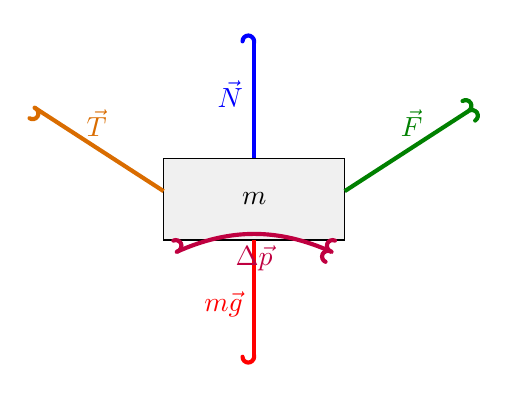
\begin{tikzpicture}[
  vector/.style={line width=1.5pt},
  label distance=2pt
]
  \draw[fill=gray!12] (-1.15,-.52) rectangle (1.15,.52);
  \node at (0,0) {$m$};
  \draw[vector,blue,-{spaced left hook}] (0,.52) -- node[left] {$\vec N$} (0,2.15);
  \draw[vector,red,-{spaced right hook}] (0,-.52) -- node[left] {$m\vec g$} (0,-2.15);
  \draw[vector,green!50!black,-{spaced hooks}] (1.15,.1) -- node[above] {$\vec F$} (2.85,1.2);
  \draw[vector,orange!85!black,-{spaced left hook reversed}]
    (-1.15,.1) -- node[above] {$\vec T$} (-2.85,1.2);
  \draw[vector,purple,{spaced right hook reversed}-{spaced hooks reversed}]
    (-1.05,-.7) to[bend left=24] node[below,sloped] {$\Delta\vec p$} (1.05,-.7);
\end{tikzpicture}
\end{document}
